\documentclass{article}

\usepackage[version=3]{mhchem}
\usepackage{siunitx}
\usepackage{natbib}
\usepackage{graphicx}
\usepackage{mathtools}
\usepackage{amssymb}
\usepackage{amsthm}
\usepackage[italian]{babel}
\usepackage{stackengine}
\usepackage{graphicx,ifthen}
\usepackage{amsmath}
\usepackage{hyperref}
\usepackage{bm}

\renewcommand{\labelenumi}{\alph{enumi}.}

\title{Esperienza I: \\ effetto fotoelettrico}
\author{Manuel G. Moretti\footnote{email: manuel.moretti560@edu.unito.it}}
\date{Luglio 2024}

\begin{document}

\maketitle

\begin{center}
\begin{tabular}{l r}
Esperimentazioni II corso B & A.A. 2023/24 \\
Modulo II & Universit\'{a} degli Studi di Torino \\
\end{tabular}
\end{center}

\begin{abstract}
In questa esperienza si è stimato il valore della costante di Planck $h$ sfruttando l'effetto fotoelettrico, in particolare illuminando un fotocatodo con cinque diodi LED di lunghezze d'onda diverse. Il valore sperimentale è stato ottenuto attraverso un fit lineare. Dopo aver effettuato un test di Gauss, il valore ottenuto è risultato compatibile co2n il valore noto dalla letteratura.
\end{abstract}

\section{Obiettivi della misura}
L'obiettivo dell'esperienza consiste nello stimare il valore della costante di Planck $h$. A questo proposito si è sfruttato l'effetto fotoelettrico, un fenomeno quantistico consistente nell'emissione di elettroni da una superficie metallica quando viene irradiata da una radiazione elettromagnetica di una frequenza non inferiore ad una certa frequenza di soglia.
\section{Configurazione dell'apparato sperimentale}
L'apparato sperimentale consiste in una scatola di metallo al cui interno sono posizionati il fotocatodo e una guida in cui posizionare i LED collegati. La scatola può essere chiusa in modo da evitare eventuali contaminazioni da parte della radiazione elettromagnetica di fondo. Ogni LED viene collegato ad un generatore di tensione, impostato a $(14.1\pm 0.1)$ V e $(0.037\pm0.001)$ A, e ad una pila da 3 V che ha la funzione di fornire la tensione di controcampo $V_c$. Variando questa tensione di controcampo si osserva una variazione delle corrente fotoelettrica, la quale viene misurata con un nanoamperometro. L'obiettivo è quello di determinare il valore di $V_c$ per cui questa corrente si annulla. 
\section{Raccolta ed elaborazione dei dati}
La raccolta dati è consistita in una serie di misure della corrente fotoelettrica in funzione della variazione della tensione di controcampo $V_c$. Il processo è stato eseguito per cinque LED diversi, di lunghezza d'onda $(472.88\pm 1.51)$ nm, $(589.88\pm1.32)$ nm, $(604.88\pm 2.33)$ nm, $(638.88\pm2.42)$ nm e $(544.38\pm 1.47)$ nm rispettivamente. 

Con i dati ottenuti è stato quindi possibile ricavare la caratteristica I-V di ognuno dei cinque LED.
\begin{figure}[h]
    \centering
    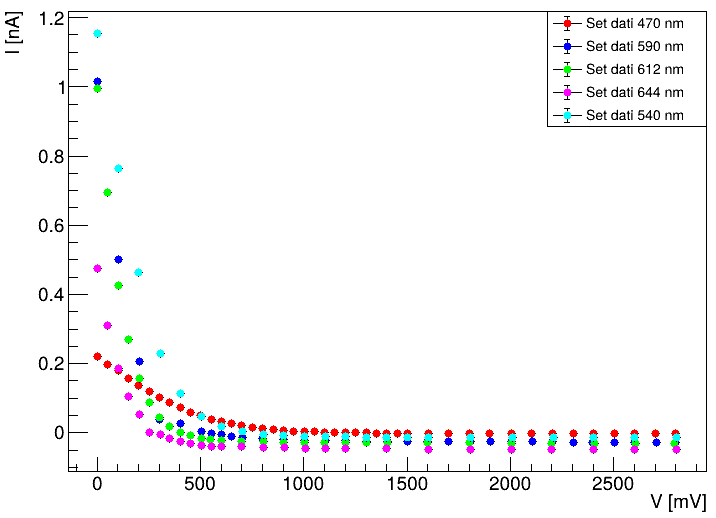
\includegraphics[width=0.8\linewidth]{Immagini/Car.LED.png}
    \caption{caratteristiche I-V dei LED}
    \label{fig:IV LEDs}
\end{figure}

Per ogni curva si è poi effettuata una regressione per ottenere il valore di $V_c$ per cui la corrente $I$ si annulla. In particolare, osservando i dati raccolti, ci si è posti nel range in cui la curva passava da valori positivi a valori negativi di $I$. In questo range di dati si è quindi effettuato un fit lineare, ovvero con una funzione del tipo $ax+b$. Per ogni retta ottenuta si è quindi potuto determinare l'intersezione con l'asse di $V$, il quale corrisponde al valore di $V_c$ interessato, indicato con $V_{c0}$.

Una volta ricavati i valori di $V_{c0}$, è possibile costruire un grafico avente come ascisse i valori della frequenza di ogni LED, ricavabili tramite la relazione $c=\lambda f$, e come ordinate i valori di $V_{c0}$ trovati.
\newpage
\begin{figure}[h]
    \centering
    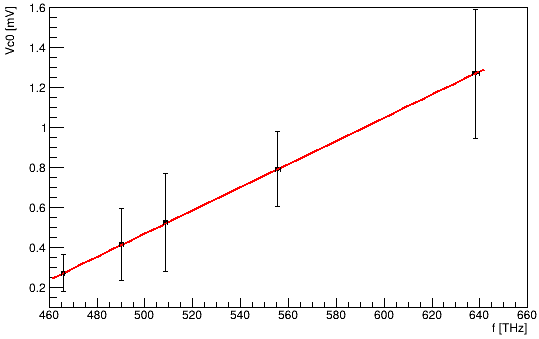
\includegraphics[width=0.7\linewidth]{Immagini/fV.png}
    \caption{grafico di $V_{c0}$ in funzione di $f$}
    \label{fig:V(f)}
\end{figure}

Si è infine effettuata sul grafico in figura \ref{fig:V(f)} una regressione lineare, in cui il valore del coefficiente angolare della retta corrisponde alla stima della costante di Planck.

\section{Risultati e conclusioni}
Dalle regressioni effettuate sul grafico in figura \ref{fig:IV LEDs} si sono ottenuti i seguenti valori di $V_{c0}$.
\begin{table}[h]
    \centering
    \begin{tabular}{|c|c|c|}
        \hline
        \bm{$\lambda_{LED}$} \textbf{[nm]} & \bm{$V_{c0}$} \textbf{[V]} & \bm{$f$} \textbf{[THz]}\\
        \hline
        $472.88\pm 1.51$ & $1.27\pm 0.32$ & $638.30\pm 1.36$ \\
        \hline
        $589.88\pm1.32$ & $0.54\pm 0.25$ & $508.48\pm 0.86$ \\
        \hline
        $604.88\pm 2.33$ & $0.42\pm 0.18$ & $490.20\pm 0.80$ \\
        \hline
        $638.88\pm2.42$ & $0.27\pm 0.09$ & $465.84\pm 0.72$ \\
        \hline
        $544.38\pm 1.47$ & $0.79\pm 0.19$ & $555.56\pm 1.03$ \\
        \hline
    \end{tabular}
    \caption{valori di $V_{c0}$}
    \label{tab:Vc0}
\end{table}

Dalla regressione effettuata dei dati in figura \ref{fig:V(f)} si è ottenuto il seguente valore di $h$
\begin{equation}
    \label{eq:stima h}
    h_s =\left(5.81\pm1.57\right)\cdot 10^{-3}\,\unit{\frac{V}{Hz}},
\end{equation}
che si è confrontato con il valore di $h$ noto
\begin{equation}
    \label{eq: h noto}
    h = \left(4.13\pm0.01\right)\cdot 10^{-3}\,\unit{\frac{V}{THz}}.
\end{equation}
Effettuando quindi un test di Gauss tra le due misure si è ottenuto un valore di $Z=0.903$, il quale è inferiore al valore critico $Z_c=1.96$ con un livello si significatività del 5\%. Le due misure sono pertanto statisticamente compatibili a seguito di quanto ottenuto con il test di Gauss. 
\end{document}